%%%%%%%%%%%%%%%%%%%%%%%%%%%%%%%%%%%%%%%%%%%%%%%%%%%%%%%%%%%%%%%%%%%%%%%%%
%%   CHAPTER: SELF-SUPPORTING SPACESHIPS
%%%%%%%%%%%%%%%%%%%%%%%%%%%%%%%%%%%%%%%%%%%%%%%%%%%%%%%%%%%%%%%%%%%%%%%%%

\renewcommand{\chapterfolder}{self_support_spaceships/}
\chapterimage{cover/self_support_spaceships}
\chapter{Self-Supporting Spaceships}\label{chp:self_support_spaceships}\index{self-supporting spaceship}


\vspace*{-0.4in}
\epigraph{Figuring out how to achieve a particular behavior makes a pleasant puzzle; actually building the thing is mostly tedious.}{Dean Hickerson}
\vspace*{0.4in}


\noindent Universal computation, covered in the previous chapter, is the first of two major types of universality that often show up in discussions of Conway's Game of Life, and cellular automata in general. The second type of universality is universal construction. Whereas universal computation is the ability to ``compute anything that can be computed'', universal construction could be loosely summarized as the ability to ``construct anything that can be constructed''.

We will cover this topic in much more depth in Chapter~\ref{chp:universal_construction}, but this chapter provides a good preview of the general idea. Indeed, in this chapter we will build spaceships that work by reaching out into a region of empty space and constructing something there. More specifically, self-supporting spaceships (the topic of this chapter) work by manipulating a reaction that moves along a track so as to construct the track in front of itself.


%%%%%%%%%%%%%%%%%%%%%%%%%%%%%%%%
\section{The Silverfish}\label{sec:silverfish}\index{silverfish}
%%%%%%%%%%%%%%%%%%%%%%%%%%%%%%%%

Most self-supporting spaceships rely on a core reaction that moves an object forward with the help of another object that is in its path. One such reaction (simply called the \emph{$31c/240$~reaction}) is displayed in Figure~\ref{fig:31c_240_reaction}, in which a Herschel collides with a block in such a way that it moves forward by $31$~cells over the course of $240$ generations.\footnote{We saw another such reaction back in Figure~\ref{fig:17c45_reaction}. We explore the consequences of this reaction a bit later, in Section~\ref{sec:caterpillar}, since building a spaceship out of it is somewhat more technical than the reaction that we use here.} At the same time, the block is moved back by $22$~cells, a second block is created, and two gliders are released.\index{31c/240 reaction}

\begin{figure}[!htb]
	\centering\embedlink{31c_240_reaction}{\vcenteredhbox{\patternimg{0.12}{31c_240_reaction_0}} \vcenteredhbox{\genarrow{240}} \vcenteredhbox{\patternimg{0.12}{31c_240_reaction_240}}}
	\caption{The $31c/240$~reaction. A Herschel collides with a block so as to move forward by $31$~cells (and move the block back by $22$~cells) over the course of $240$~generations. This reaction also produces a second block (at the top-center) and two gliders as by-products.}\label{fig:31c_240_reaction}
\end{figure}

The first major goal of this chapter is to use this reaction to create a $31c/240$ spaceship, which we call the \emph{silverfish}. The major obstacles that we will have to overcome are cleaning up the extra objects (blocks and gliders) left behind by the Herschel as it moves, and using the Herschel to create a block in front of itself before it gets there.


\subsection{Herschel Crawlers and Rakes}\label{sec:silverfish_herschel_crawler}

If we place blocks in a straight line with a spacing of $31$ cells, a Herschel is able to crawl along them (via the $31c/240$ reaction of Figure~\ref{fig:31c_240_reaction}) at a speed of $31c/240$. Furthermore, if we place two of these tracks next to each other, we can use one of the output gliders from one of the Herschels to cleanly erase the extra block that is produced by the other Herschel, as illustrated in Figure~\ref{fig:31c_240_herschel_pair}. When we do this, we get a track for two Herschels called a \emph{reburnable wick}:\index{reburnable wick} a wick that is not used up (but is potentially repositioned and/or rephased) after its fuse (the pair of Herschels) burns through it.

\begin{figure}[!htb]
	\centering
	\patternimglink{0.0885}{31c_240_herschel_pair}
	\caption{A reburnable block wick, along which a pair of Herschels (highlighted in \bgbox{greenpastel}{green}) can move at a speed of $31c/240$. The spark and blocks highlighted in \bgbox{redback}{red} are only temporary---they are destroyed as the Herschels move farther down the track.}\label{fig:31c_240_herschel_pair}
\end{figure}

While a single Herschel pair changes the positions of the blocks in the reburnable wick, a sequence of 31 Herschel pairs would leave them all exactly where they would be if no Herschels burned through them at all.\footnote{After the $31$ Herschel pairs burned through them, each block would actually be moved back $22 \times 31 = 682$ cells. However, since the wick is infinitely long and the blocks are spaced $31$~cells apart, this makes no difference.} This gives us an infinitely-long pattern that moves at a speed of $31c/240$. We now focus on converting this pattern into a \emph{finite} configuration (i.e., a spaceship) that moves at the same speed.

To this end, we need a way of constructing the blocks in front of the Herschel pairs that burn through them. Fortunately, blocks are fairly easy to construct---we can collide spaceships like gliders together so as to synthesize them. Furthermore, the Herschel pairs create gliders as they move, so we ``just'' need to redirect those gliders in front of the Herschels so as to synthesize the blocks.

Unfortunately, getting gliders (or any other spaceships) in front of the Herschel pair is quite tricky, as it does not seem like it should be possible to reflect the gliders that the Herschel pair emits without making use of stationary components like Snarks or other small spaceships (none of which travel at $31c/240$). One technique that works to at least let us send gliders forward (instead of backward, as in Figure~\ref{fig:31c_240_herschel_pair}) is to use the two-glider kickback reaction from Table~\ref{tab:2_glider_synth}. Unfortunately, to make use of this reaction, we have to place even more of these tracks next to each other. One configuration that works is displayed in Figure~\ref{fig:31c_240_forward_rake}---it makes use of six Herschels and six block tracks instead of just two.

We call this pattern a \emph{forward rake}\index{forward rake} even though it is not \emph{technically} a rake due to its reliance on the supporting block tracks. Since firing gliders backward via these Herschels is so straightforward (they fire gliders backward all on their own, after all), it is not difficult to construct the \emph{backward rake}\index{backward rake} in Figure~\ref{fig:31c_240_back_rake} that works on this same set of six block tracks (instead of the one that works on two block tracks, which we saw in Figure~\ref{fig:31c_240_herschel_pair}).

These rakes have one big limitation, however---we can only use them to place an output glider on every $31$st lane. If we want to make sure that a glider is fired on a \emph{particular} lane, we need a mechanism for moving the block track (and thus any subsequent rakes) slightly forward or backward. Fortunately, this is also straightforward---the \emph{rephaser} displayed in Figure~\ref{fig:31c_240_rephaser} moves the block tracks backward by $22$~cells (or equivalently, forward by $9$~cells) simply by having a Herschel burn through each track in such a way that their output gliders annihilate one another. Importantly, since $\mathrm{gcd}(22,31) = 1$, we can use multiple copies of this rephaser so as to make subsequent rakes output gliders on any lanes of our choosing.

\begin{figure}[!htb]
	\centering
	\begin{subfigure}{0.28\textwidth}
		\centering
		\embedlink{31c_240_rakes_and_rephaser}{\gridbox{0.5pt}{\patternimg{0.072}{31c_240_back_rake}}}
		\caption{A backward rake.}\label{fig:31c_240_back_rake}
	\end{subfigure} \ \ \begin{subfigure}{0.28\textwidth}
		\centering
		\patternlink{31c_240_rakes_and_rephaser}{\gridbox{0.5pt}{\patternimg{0.072}{31c_240_rephaser}}}
		\caption{A rephaser.}\label{fig:31c_240_rephaser}
	\end{subfigure} \ \ \begin{subfigure}{0.4\textwidth}
		\centering
		\patternlink{31c_240_rakes_and_rephaser}{\gridbox{0.5pt}{\patternimg{0.072}{31c_240_forward_rake}}}
		\caption{A forward rake.}\label{fig:31c_240_forward_rake}
	\end{subfigure}
	\caption{Rakes and rephasers that crawl along $6$ reburnable block wicks at a speed of $31c/240$. In each case, the $6$ Herschels release $12$ gliders every $240$~generations, and $6$ of those gliders are used to destroy the excess blocks left behind by each Herschel. In (a) the backward rake, $4$ of the gliders collide so as to destroy each other and the other $2$ are released backward. In (b) the rephaser, $2$ gliders are destroyed in a kickback reaction and then the other $4$ are destroyed by colliding into each other. In (c) the forward rake, $4$ kickback reactions are used to destroy $4$ of the gliders, leaving the remaining $2$ gliders to escape to the front.}\label{fig:31c_240_rakes_and_rephaser}
\end{figure}


\subsection{Synthesizing and Destroying Block Tracks}\label{sec:silverfish_synth_destroy_blocks}

Fortunately, even though we now have $6$ block tracks, the problem of constructing the blocks in front of the Herschels is not much trickier than it was when we just had $2$ block tracks. Indeed, we can construct $4$ of these block tracks simply via these rakes and some additional kickback reactions, as illustrated in Figure~\ref{fig:31c_240_track_builder}.

While it lining up these kickback reactions and block syntheses is somewhat tricky due to the difficulty of controlling which lanes we produce gliders on when using these tracks, we fortunately have complete control of the \emph{timing} of the gliders on these lanes. Indeed, by delaying Herschels appropriately (and perhaps adding a single row of blocks to a track so as to change the color of the gliders that a Herschel produces) we can create any $2$-glider collision that we like. By using this technique, we can clean up these six block tracks just by using even more kickback reactions, as illustrated in Figure~\ref{fig:31c_240_track_destroyer}.

\begin{figure}[!htbp]
	\centering
	\begin{subfigure}{\textwidth}
		\centering
		\embedlink{31c_240_track_builder}{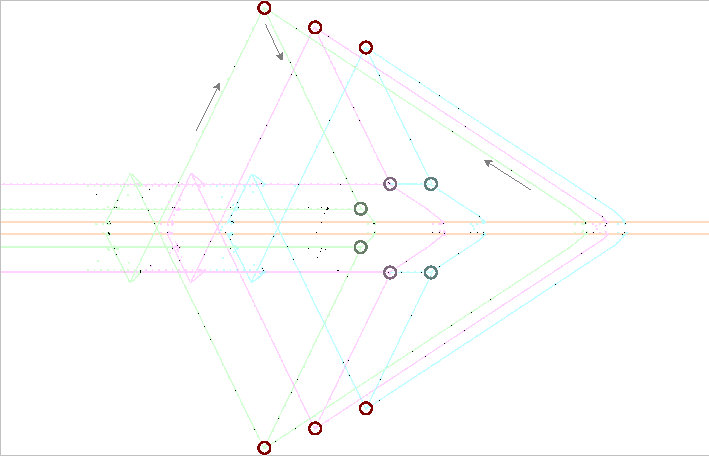
\includegraphics[width=\textwidth]{self_support_spaceships/31c_240_track_builder.pdf}}
		\caption{A configuration of rakes that turns a $2$-block track (highlighted in \bgbox{orangeback2}{orange}) into a $6$-block track.}\label{fig:31c_240_track_builder}
	\end{subfigure} \\[0.2cm]
	\begin{subfigure}{\textwidth}
		\centering
		\embedlink{31c_240_track_destroyer}{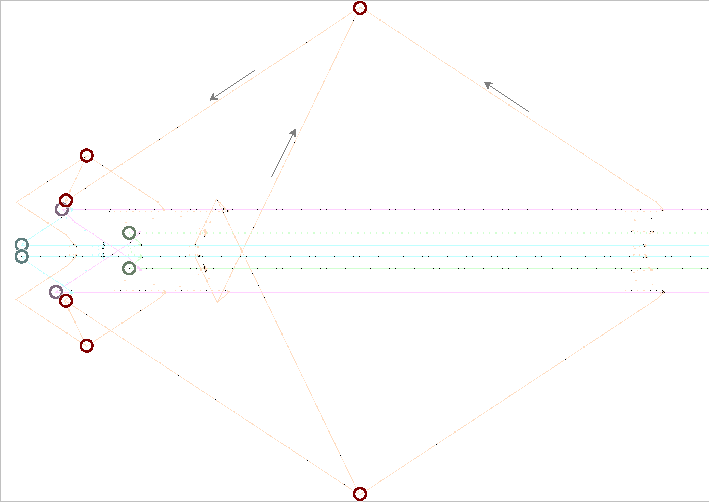
\includegraphics[width=\textwidth]{self_support_spaceships/31c_240_track_destroyer.pdf}}
		\caption{A configuration of rakes that destroys the $6$-block track. Destroying the tracks is actually straightforward, but multiple kickback reactions must be used to clean up the leftover gliders (highlighted in \bgbox{orangeback2}{orange}).}\label{fig:31c_240_track_destroyer}
	\end{subfigure} \\
	\caption{A configuration of rakes that uses multiple kickback reactions (circled in \bgbox{redback}{red}) to position gliders so that they can either (a) synthesize block tracks ahead of the rakes, or (b) destroy the block tracks behind the rakes. The locations where gliders synthesize or destroy the block tracks are circled near the center.}\label{fig:31c_240_builder_destroyer}
\end{figure}

However, we still do not have a method of constructing the two central block tracks at the front of Figure~\ref{fig:31c_240_track_builder}, since there is no way to arrange kickback reactions so as to put gliders in front of the frontmost rakes. While this may seem like an insurmountable problem at first, one solution is to synthesize light, middle, and/or heavyweight spaceships that travel in the same direction as the Herschels, and then bounce gliders off of those rows of xWSSs.

While this approach works, instead of bouncing a glider back toward the front of the Herschels so as to synthesize the block track, we convert that glider into a middleweight spaceship via the reaction illustrated in Figure~\ref{fig:g_2h_to_m}. The reason for this is that a middleweight spaceship can stabilize the front of the Herschel track in the exact same way as a block (in fact, one of the Herschel's sparks simply converts the MWSS into a block in the correct position), as illustrated in Figure~\ref{fig:herschel_mwss_stabilize}.

\begin{figure}[!htb]
	\centering
	\begin{subfigure}[b]{0.43\textwidth}
		\centering
		\embedlink{g_2h_to_m}{\vcenteredhbox{\patternimg{0.132}{g_2h_to_m}} \vcenteredhbox{\genarrow{38}} \vcenteredhbox{\patternimg{0.132}{g_2h_to_m_38}}}
		\caption{A way of colliding a glider with two heavyweight spaceships so as to make a perpendicular middleweight spaceship.}\label{fig:g_2h_to_m}
	\end{subfigure} \ \	\ \ \begin{subfigure}[b]{0.53\textwidth}
		\centering
		\embedlink{herschel_mwss_stabilize}{\vcenteredhbox{\patternimg{0.075}{herschel_mwss_stabilize}} \vcenteredhbox{\genarrow{98}} \vcenteredhbox{\patternimg{0.075}{herschel_mwss_stabilize_98}} \vcenteredhbox{\genarrow{142}} \vcenteredhbox{\patternimg{0.075}{herschel_mwss_stabilize_240}}}
		\caption{An MWSS stabilizing a Herschel crawler.}\label{fig:herschel_mwss_stabilize}
	\end{subfigure}
	\caption{Some reactions that can be used to stabilize the front of the $31c/240$ Herschel crawler, as long as we can somehow create a parallel double stream of heavyweight spaceships.}\label{fig:silverfish_mwss_reactions}
\end{figure}

The last remaining question before we can piece together all of these reactions is how to create the pair of heavyweight spaceships that are used in Figure~\ref{fig:g_2h_to_m}. The key insight that makes this possible is the fact that we can fire a glider at an HWSS so as to create some debris without affecting the HWSS (after all, heavyweight spaceships are nice and sparky), and then we can fire additional gliders at that debris so as to create a HWSS.\footnote{In a sense, we are using a heavyweight spaceship to synthesize itself. It is this self-creation that is really what makes it possible to turn the $31c/240$ reaction into a spaceship.} One reaction that implements the first half of this process, by creating a toad and a beehive a safe distance from the HWSS when a pair of gliders hits it (without disturbing the HWSS\footnote{That is, this reaction is a Heisenburp.}\index{Heisenburp}), is displayed in Figure~\ref{fig:hwss_toad_beehive}. An unfortunate feature of this reaction is that it relies on two synchronized gliders, and synchronizing the precise time and (especially) position of multiple gliders that are fired from these block tracks is quite tricky. Nevertheless, this synchronization is possible via kickback reactions, and one configuration of rakes that produces the exact glider pair that we need is displayed in Figure~\ref{fig:31c_240_double_gun}.

\begin{figure}[!htb]
	\centering
	\begin{subfigure}[b]{0.28\textwidth}
		\centering
		\embedlink{hwss_toad_beehive}{\begin{tikzpicture}[rotate=-90,transform shape]%
			\node[inner sep=0pt,anchor=south west] (dg) at (0,0) {\vcenteredhbox{\patternimg{0.093}{hwss_toad_beehive_0}} \vcenteredhbox{{\color{black}$\xrightarrow{\scriptsize\rotatebox[origin=c]{90}{\text{\clock{2}{40} 160}}}$}} \vcenteredhbox{\patternimg{0.093}{hwss_toad_beehive_160}}};
			\end{tikzpicture}}
		\caption{A way of colliding two gliders with an HWSS so as to make a beehive and a toad away from the HWSS stream, and without affecting the HWSS.}\label{fig:hwss_toad_beehive}
	\end{subfigure} \ \	\ \ \begin{subfigure}[b]{0.69\textwidth}
		\centering
		\embedlink{31c_240_double_gun}{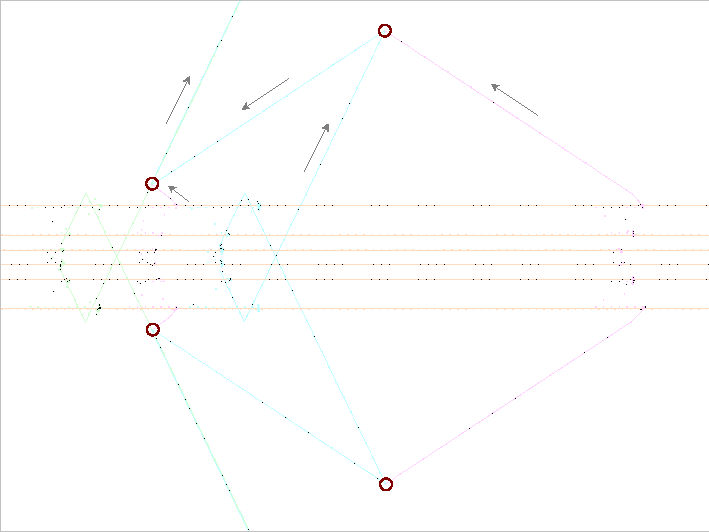
\includegraphics[width=\textwidth]{self_support_spaceships/31c_240_double_gun.pdf}}
		\caption{A configuration of block-crawling rakes that uses some kickback reactions (circled in \bgbox{redback}{red}) to create the synchronized $2$-glider paired needed in (a).}\label{fig:31c_240_double_gun}
	\end{subfigure}
	\caption{The configuration of rakes in (b) sends out a pair of gliders that, when they collide with a heavyweight spaceship as in (a), produce a beehive and a toad. That beehive and toad can then be used as a seed for a slow-salvo synthesis of that heavyweight spaceship.}\label{fig:31c_240_double_gun_at_hwss}
\end{figure}

There are numerous different ways that we could fire gliders at that toad and beehive so as to turn them into a heavyweight spaceship. For the sake of simplicity, we use a slow salvo, since synchronizing the precise time and (especially) position of multiple gliders that are fired from these block tracks is quite tricky (as we saw for just two gliders in Figure~\ref{fig:31c_240_double_gun}). We furthermore just use gliders coming from one of the four possible directions, since (a) the gliders are fired from the $6$-block track, which restricts us to just two directions (i.e., from forward and backward rakes on the block track), and (b) if we further restrict to gliders just coming from forward rakes then it makes the resulting construction of the $31c/240$ spaceship somewhat simpler and more uniform.\footnote{Point (b) here is somewhat subjective---allowing gliders from backward rakes would decrease the number of gliders required, but perhaps increase the spacing needed between the rakes and make their placement somewhat more complicated. See Exercise~?? for an example of how backward gliders might be useful.} One particular slow salvo of this type that works is displayed in Figure~\ref{fig:hwss_from_toad_beehive}.\footnote{This recipe was produced by a long-running breadth-first search using a script that was written by ConwayLife.com forums user ``oblique''---see \httpsurl{conwaylife.com/forums/viewtopic.php?t=1296}. It was one of the first options to show up that produced an upward HWSS with enough clearance that other HWSSes could safely travel past all the intermediate stages of the slow-salvo construction. It is not necessarily the smallest unidirectional salvo that exists, but it is probably fairly close.}


\subsection{Glider Lanes and More Rakes}\label{sec:silverfish_more_rakes}

At this point, we have essentially everything that we need to construct a $31c/240$ spaceship. However, the spaceship that results from combining the various reactions and patterns that we have developed in this section ends up being monstrously large, so it is worthwhile to spend some time thinking about how we can reduce its size prior to assembling it.

The majority of this spaceship's length will come from the multi-step process needed to synthesize the heavyweight spaceship pair on each of its sides via the slow salvo of Figure~\ref{fig:hwss_from_toad_beehive}.\footnote{Similarly, the majority of its width comes from how close to the front of the spaceship we can put the first forward rake.} Indeed, implementing this synthesis requires $13$ gliders and thus $13$ forward rakes. Furthermore, we need to use between $0$ and $30$ rephasers before each of those rakes to make sure the gliders that they emit are positioned on the correct mod~$31$ lane.

\begin{figure}[!htb]
	\centering\raisebox{-0.49\height}{\begin{tikzpicture}[scale=0.5, every node/.style={transform shape}]%
		\node[inner sep=0pt,anchor=south west] at (0,0) {\embedlink{hwss_from_toad_beehive}{\patternimg{0.182}{hwss_from_toad_beehive}}};
		
		\colorletternode{green}{9.89}{6.3}{1}
		\colorletternode{green}{10.43}{10.8}{2}
		\colorletternode{green}{8.77}{8.53}{3}
		\colorletternode{green}{7.88}{7.7}{4}
		\colorletternode{green}{9.16}{5.05}{5}
		\colorletternode{green}{6.68}{7.48}{6}
		\colorletternode{green}{8.08}{4.49}{7}
		\colorletternode{green}{5.07}{8.45}{8}
		\colorletternode{green}{6.08}{5.81}{9}
		\colorletternode{green}{7.21}{3.3}{10}
		\colorletternode{green}{4.45}{5.42}{11}
		\colorletternode{green}{3.14}{5.83}{12}
		\colorletternode{green}{6.12}{2.63}{13}
		\end{tikzpicture}} \patternlink{hwss_from_toad_beehive}{\vcenteredhbox{\gliderarrow{13}} \vcenteredhbox{\patternimg{0.091}{hwss_from_toad_beehive_13}}}
	\caption{A $13$-glider slow salvo that turns the configuration of a beehive and toad from Figure~\ref{fig:hwss_toad_beehive} back into an HWSS on the same lane as the HWSS that was used to create them.}\label{fig:hwss_from_toad_beehive}
\end{figure}

In order to reduce the number of rephasers needed, and thus reduce the spaceship's length, we now introduce several other forward rakes that emit gliders on different lanes. These rakes, which are displayed in Figure~\ref{fig:31c_240_forerakes},\footnote{This collection of rakes is by no means exhaustive. See Exercises~\ref{exer:self_support_spaceships_r4l1}--\ref{exer:self_support_spaceships_r3l28}, and there are many others known as well (and probably quite a few others waiting to be found). The rakes given in Figure~\ref{fig:31c_240_forerakes} are pretty good at hitting each mod~$31$ lane efficiently, though.} work in one of three different ways:\smallskip

\begin{itemize}
	\item by using multiple copies of the two-glider kickback reaction (as in Figure~\ref{fig:R6L17}),\footnote{Each pair of kickback reactions that we use in this way has the net effect of adding $2$ rephaser lengths to the rake and increasing its output lane number by $16$ (mod $31$)---see Exercise~\ref{exer:self_support_spaceships_r4l1}.}\smallskip
	
	\item by using the two-glider synthesis of a traffic light and a glider from Table~\ref{tab:2_glider_synth}, and then using another glider or two to clean up the traffic light (as in Figure~\ref{fig:R6L6}), or\smallskip
	
	\item by using two gliders to synthesize a small object that can be used to release a glider on another lane when it is destroyed (as in Figures~\ref{fig:31c_240_forerakes}(a) and~(b)).\smallskip
\end{itemize}

In order to help us keep track of where each of these rakes emits a glider, we name them according to what mod~$31$ lane they fire a glider on (relative to the original forward rake that we saw in Figure~\ref{fig:31c_240_forward_rake}, which we say fires on lane~$0$) and the number of Herschels that are used on each block track. Specifically, their names have the form
\[
\text{\texttt{R<number of Herschels>L<lane number>}},
\]
so that the original rake from Figure~\ref{fig:31c_240_forward_rake}, for example, is called \texttt{R1L0} (it uses a single Herschel on each block track and produces a glider on lane~0).\footnote{The ``\texttt{R}'' in this naming scheme stands for the fact that the rake has approximately the same length as this number of \textbf{r}ephasers, and the ``\texttt{L}'' stands for ``\textbf{l}ane''.}

\begin{figure}[!htb]
	\centering
	\begin{minipage}{0.3\textwidth}
		\begin{subfigure}{\linewidth}
			\centering
			\gridbox{0.5pt}{\patternimglink{0.0975}{R2L23}}
			\caption{\texttt{R2L23}\index{R2L23}}\label{fig:R2L23}
		\end{subfigure} \\[0.1cm] \begin{subfigure}{\linewidth}
			\centering
			\gridbox{0.5pt}{\patternimglink{0.0975}{R2L25}}
			\caption{\texttt{R2L25}\index{R2L25}}\label{fig:R2L25}
		\end{subfigure}
	\end{minipage} \ \ \ \begin{subfigure}{0.66\textwidth}
		\centering
		\gridbox{0.5pt}{\patternimglink{0.072}{R6L17}}
		\caption{\texttt{R6L17}\index{R6L17}}\label{fig:R6L17}
	\end{subfigure} \\[0.1cm]
	\begin{subfigure}{0.3\textwidth}
		\centering
		\gridbox{0.5pt}{\patternimglink{0.0975}{R1L0}}
		\caption{\texttt{R1L0}\index{R1L0}}\label{fig:R1L0}
	\end{subfigure} \ \ \ \begin{subfigure}{0.66\textwidth}
		\centering
		\gridbox{0.5pt}{\patternimglink{0.06444285714}{R6L6}}
		\caption{\texttt{R6L6}\index{R6L6}}\label{fig:R6L6}
	\end{subfigure}
	\caption{Several forward rakes that crawl along a six-block track and emit gliders on different lanes mod~$31$. The forward rake from Figure~\ref{fig:31c_240_forward_rake} is the one displayed here at the bottom-left, called \texttt{R1L0}.}\label{fig:31c_240_forerakes}
\end{figure}

The ``\texttt{R}'' piece of this naming scheme is useful both as a measure of how long the rake is (e.g., it tells us that \texttt{R6L17} is roughly three times as long as \texttt{R2L25}) and also for computing the mod~$31$ output glider lane of subsequent rakes. Indeed, a single rephaser (i.e., one Herschel on each block track) changes the output lane of subsequent gliders by $-22$ (or equivalently, by $+9$) mod $31$, so a rake with name \texttt{R<m>L<n>} adjusts the output lane of subsequent gliders by $+9m$ (mod $31$). For example, \texttt{R6L21} increases the output lane of subsequent gliders by $9 \times 6 = 54 \equiv 23$ (mod $31$).

With these rakes in hand, we can fire gliders on particular mod~$31$ lanes much more efficiently than we could previously. For example, placing a glider on lane~$22$ (when the block track is currently aligned to lane~$0$) via just the rakes and rephaser from Figure~\ref{fig:31c_240_rakes_and_rephaser} would require $30$~rephasers followed by the forward rake \texttt{R1L0}. However, a much more efficient way of firing a glider on lane~$22$ is to use just $4$~rephasers and then the forward rake \texttt{R6L17} (for a total length of $4 + 6 = 10$ Herschels per track, instead of $30 + 1 = 31$ Herschels per track). A summary of the most efficient rake to use to place a glider on each mod~$31$ lane is provided in Table~\ref{tab:silverfish_forward_rakes}.

\begin{table}[!htbp]
	\centering
	\begin{tabular}{c l | c l | c l | c l}
		\toprule
		Lane & Cheapest Rake & Lane & Rake & Lane & Rake & Lane & Rake \\ \midrule
		0 & \texttt{R1L0} & 9 & 1 + \texttt{R1L0} & 18 & 2 + \texttt{R1L0} & 27 & 3 + \texttt{R1L0} \\
		1 & 1 rephaser + \texttt{R2L23} & 10 & 2 + \texttt{R2L23} & 19 & 3 + \texttt{R2L23} & 28 & 4 + \texttt{R2L23}\\
		2 & 3 rephasers + \texttt{R6L6} & 11 & 4 + \texttt{R6L6} & 20 & 5 + \texttt{R6L6} & 29 & 6 + \texttt{R6L6} \\
		3 & 1 rephaser + \texttt{R2L25} & 12 & 2 + \texttt{R2L25} & 21 & 3 + \texttt{R2L25} & 30 & 4 + \texttt{R2L25} \\
		4 & 2 rephasers + \texttt{R6L17} & 13 & 3 + \texttt{R6L17} & 22 & 4 + \texttt{R6L17} & & \\
		5 & 4 rephasers + \texttt{R1L0} & 14 & 5 + \texttt{R1L0} & 23 & \texttt{R2L23} & & \\
		6 & \texttt{R6L6} & 15 & 1 + \texttt{R6L6} & 24 & 2 + \texttt{R6L6} & & \\
		7 & 7 rephasers + \texttt{R6L6} & 16 & 8 + \texttt{R6L6} & 25 & \texttt{R2L25} & & \\
		8 & 5 rephasers + \texttt{R2L25} & 17 & \texttt{R6L17} & 26 & 1 + \texttt{R6L17} & & \\
		\bottomrule
	\end{tabular}
	\caption{A summary of the shortest forward rakes that can be used to put a glider on a given lane (mod $31$). For example, the shortest configuration of rephasers and forward rakes that can put a glider on lane~22 (when currently aligned to lane~0) consists of 4 rephasers followed by \texttt{R6L17}. Indeed, that configuration has a total length that is roughly the same as that of $6 + 4 = 10$ rephasers, and no other way of using rephasers and forward rakes is shorter.}\label{tab:silverfish_forward_rakes}
\end{table}


\subsection{Completing the Silverfish}\label{sec:silverfish_completed}

We now proceed with construction of the silverfish. At the front of the spaceship we use the track-building component that we built in Figure~\ref{fig:31c_240_track_builder} (with the understanding that we will still have to construct the two central block tracks somehow), and at the back of the spaceship we use the track-destroying component that we built in Figure~\ref{fig:31c_240_track_destroyer}. Right behind the track-building component, we place a forward rake that is aimed at a parallel stream of heavyweight spaceship pairs as in Figure~\ref{fig:g_2h_to_m}, which create middleweight spaceships to stabilize the two central block tracks as in Figure~\ref{fig:herschel_mwss_stabilize}.

The remainder of the silverfish is made up of forward rakes that synthesize the stream of heavyweight spaceship pairs, using the mechanisms of Figures~\ref{fig:31c_240_double_gun_at_hwss} and~\ref{fig:hwss_from_toad_beehive}. Indeed, after using the double gun from Figure~\ref{fig:31c_240_double_gun} to create a beehive and toad, we want to create $13$~gliders on the following sequence of lanes, as indicated by Figure~\ref{fig:hwss_from_toad_beehive}:\footnote{We actually have some flexibility in which lanes we use here---see Exercise~\ref{exer:silverfish_list_of_lanes}.}\label{page:silverfish_lanes}
\[
\text{\texttt{0, 11, 8, 7, 29, 13, 1, 19, 8, 0, 14, 22, 2}.}
\]
We can place gliders on these lanes by repeatedly using Table~\ref{tab:silverfish_forward_rakes} and keeping track of what lane the block tracks are currently synchronized to. After the two-glider rake from Figure~\ref{fig:31c_240_double_gun}, the block tracks are synchronized to lane~7. We then place $13$ more rakes as follows:\smallskip

\begin{itemize}
	\item First, we want to fire a glider 24 (mod~31) lanes up from the current lane, on lane~0. Table~\ref{tab:silverfish_forward_rakes} tells us that the most efficient way to do this is to use $2$~rephasers and then \texttt{R6L6}. Since this places $8$ Herschels on each track, it synchronizes the block tracks to lane $7 + (9 \times 8) = 79 \equiv 17$ (mod~$31$).\smallskip
	
	\item Next, we want to fire a glider $6$ lanes down (i.e., $25$ lanes up) from here on lane $11$ mod $31$. Table~\ref{tab:silverfish_forward_rakes} tells us that the most efficient way to do this is to use \texttt{R2L25}. Since this places $2$ Herschels on each track, it synchronizes the tracks to lane $17 + (9 \times 2) = 35 \equiv 4$ (mod~$31$).\smallskip
	
	\item Next, we want to fire a glider $4$ lanes up from here on lane $8$. Table~\ref{tab:silverfish_forward_rakes} tells us that the most efficient way to do this is to use $2$~rephasers followed by \texttt{R6L17}. Since this places $8$ Herschels on each track, it synchronizes the tracks to lane $4 + (9 \times 8) = 76 \equiv 14$ (mod~$31$).\smallskip
\end{itemize}

If we continue in this way, we quickly arrive at the following sequence of rakes and rephasers that should be placed along the $6$-block track so as to synthesize one of the heavyweight spaceships that we need beside it:\footnote{The timing of most of these rakes and rephasers does not matter, so we can simply pack them as tightly together as possible. However, the final \texttt{R6L6} has to be delayed slightly so that the HWSS it created arrives at the front double rake at the correct time.}\label{page:silverfish_rake_seq}
\begin{gather*}
	\text{\texttt{double rake, 2 rephasers, R6L6, R2L25, 2 rephasers, R6L17, 2 rephasers, R6L6,}} \\
	\text{\texttt{4 rephasers, R1L0, R6L6, 3 rephasers, R6L6, 1 rephaser, R2L23, R2L25,}} \\
	\text{\texttt{4 rephasers, R2L25, 3 rephasers, R2L25, 1 rephaser, R6L6, R2L25.}}
\end{gather*}

If we use two copies of this entire sequence of rakes and rephasers (since we need to synthesize two heavyweight spaceships on each side of the block track), we finally get a complete $31c/240$ orthogonal spaceship,\footnote{Created by Chris Cain, Dave Greene, and Adam P. Goucher in May 2020.} which is displayed in Figure~\ref{fig:silverfish}. Despite its massive size of $215{\thousep}338$ live cells and $11{\thousep}970 \times 48{\thousep}047$ bounding box, it is the smallest known $31c/240$ spaceship.\footnote{Actually, there are some modifications of it that can reduce its size a bit---see Exercise~\ref{exer:silverfish_backward_glider_destroy}.}

\begin{figure}[!htbp]
	\centering
	\embedlink{silverfish}{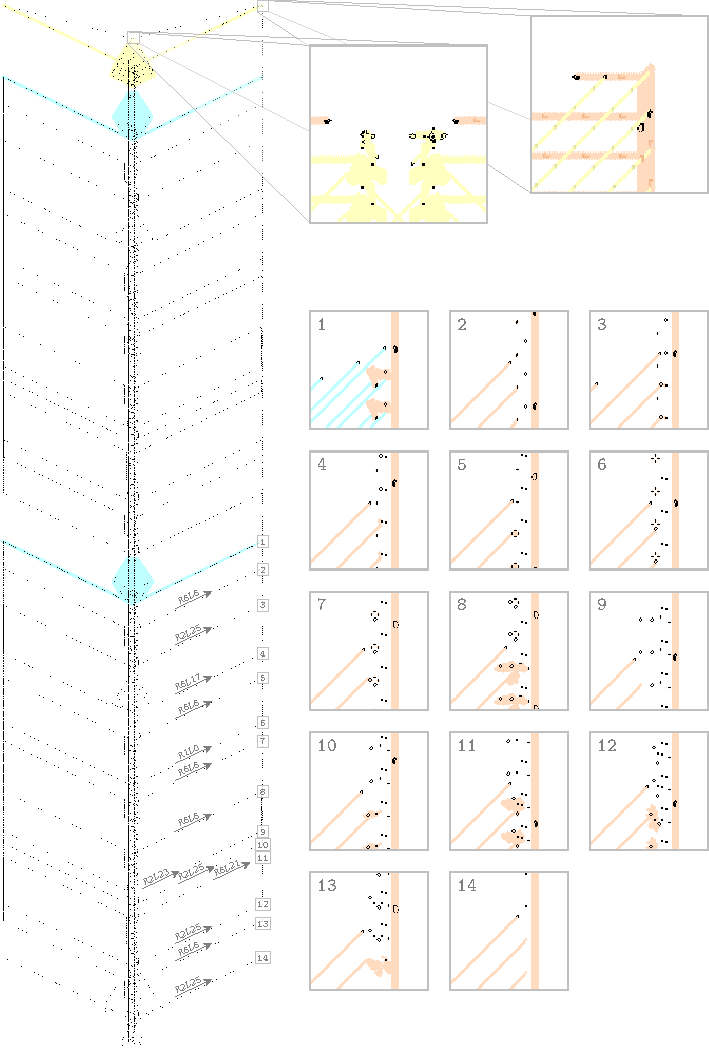
\includegraphics[width=\textwidth]{self_support_spaceships/silverfish.pdf}}
	\caption{The \emph{silverfish}: a $31c/240$ orthogonal spaceship oriented so that it travels up. The track-building mechanism from Figure~\ref{fig:31c_240_track_builder} is highlighted in \bgbox{yellowback2}{yellow}, a track-destroying mechanism like the one from Figure~\ref{fig:31c_240_track_destroyer} is highlighted in \bgbox{magentaback}{magenta}, and the double-glider forward rakes from Figure~\ref{fig:31c_240_double_gun} are highlighted in \bgbox{aquaback}{aqua}. The remaining un-highlighted rakes implement the 13-step slow salvo synthesis of a heavyweight spaceship from Figure~\ref{fig:hwss_from_toad_beehive}.}\label{fig:silverfish}
\end{figure}


% Nivasch article: http://www.gabrielnivasch.org/fun/life/caterpillar
%%%%%%%%%%%%%%%%%%%%%%%%%%%%%%%%
\section{The Caterpillar}\label{sec:caterpillar}\index{caterpillar}
%%%%%%%%%%%%%%%%%%%%%%%%%%%%%%%%

We saw another reaction that can be used to construct a self-supporting spaceship way back in Figure~\ref{fig:17c45_reaction}: a blinker can be used to move a pi-heptomino forward by $17$~cells over the course of $45$~generations (while just repositioning, not destroying, the blinker). By placing a row of blinkers with a spacing of $17$~cells as in Figure~\ref{fig:reburnable_blinker_wick}, we thus get a reburnable blinker wick that a pi-heptomino can burn through.

\begin{figure}[!htb]
	\centering
	\patternimglink{0.075}{reburnable_wick}
	\caption{A reburnable blinker wick, along which a pi-heptomino fuse (highlighted in \bgbox{greenpastel}{green}) can move at a speed of $17c/45$. The cells highlighted in \bgbox{redback}{red} make up a large spark that simply dies without affecting anything else.}\label{fig:reburnable_blinker_wick}
\end{figure}

% Redo the next 2 paragraphs in light of earlier Silverfish

A single pi-heptomino shifts the blinker wick backward by $6$~cells and rephases it,\footnote{Since the blinker wick is infinitely long, it is perhaps better to think of the pi-heptomino as shifting the wick forward by $11$~cells and not rephasing it} so if we were to place 34 pi-heptominoes on this reburnable wick then it would be moved back by $6 \times 34 = 204$ cells (which, due to the spacing of the blinkers, leaves them all exactly where they would be if no pi-heptominoes burned through them at all).\footnote{If we used just $17$ pi-heptominoes instead, the blinkers would return to their original positions, but in the opposite phases.} This gives us an infinitely-long pattern that moves at a speed of $17c/45$---our goal is to turn this into a finite configuration (i.e., a spaceship) that moves at the same speed (just like we turned the Herschel-crawling reaction of Figure~\ref{fig:31c_240_herschel_pair} into a $31c/240$ spaceship).

To this end, we need a way of constructing the blinkers in front of the pi-heptominoes that burn through them, and also a way of cleaning them up behind those pi-heptominoes. Fortunately, most of the same ideas that we used when constructing the silverfish still apply: we can use multiple pi-heptominoes on multiple reburnable blinker wicks to create rakes, we can use kickback reactions to clean up the blinker trails, and we can use parallel xWSS streams to help us synthesize the front ends of the blinker wicks.

Most of the details of this construction are quite similar to what they were for the $31c/240$ silverfish, so we omit many of the details. Instead, we just focus on two parts of the construction where the details do change considerably.


\subsection{Pi-Crawler Rakes}\label{sec:caterpillar_pi_rakes}\index{pi crawler}

The first key difference between the Herschel crawler of Figure~\ref{fig:31c_240_herschel_pair} and the pi crawler that we are now using is that the pi crawler does not emit any gliders on its own. Fortunately, it does create a large spark, and we can collide two of those sparks without much effort so as to create a backward rake, as illustrated in Figure~\ref{fig:pi_backward_rake}. Creating a forward rake that travels along this same pair of blinker tracks is a bit trickier, but can be done via six pi crawlers (three per track), as in Figure~\ref{fig:pi_forward_rake}.

\begin{figure}[!htbp]
	\centering
	\begin{tabular}{@{}cc@{}}
		\begin{subfigure}{0.44\textwidth}
			\patternimglink{0.099}{pi_backward_rake}
			\caption{A backward pi-crawler rake.}\label{fig:pi_backward_rake}
		\end{subfigure} &
		\begin{subfigure}{0.535\textwidth}
			\patternimglink{0.099}{pi_forward_rake}
			\caption{A forward pi-crawler rake.}\label{fig:pi_forward_rake}
		\end{subfigure}
	\end{tabular}
	\caption{A pair of p$45$ (a) backward and (b) forward rakes that crawl along a pair of blinker tracks that are separated by $32$~cells.}\label{fig:pi_rakes}
\end{figure}

While the blinker tracks that these rakes use have the same spacing as each other ($32$ cells), the relative phases of those blinker tracks are different. As a result, it is not possible to place a forward rake directly behind a backward rake, or vice-versa, unless we rephase one of the tracks. Fortunately, we can always properly rephase the tracks by simply inserting additional pi crawlers on one of them, since $\mathrm{gcd}(11,34) = 1$.\footnote{This is directly analogous to how we could always properly rephase the six-block track in the silverfish since $\mathrm{gcd}(9,31) = 1$.}

With that technicality out of the way, we can then place a forward rake on the same pair of tracks behind a backward rate so that their gliders collide and synthesize other objects. For example, we can use these rakes to synthesize and/or destroy additional blinker tracks, as illustrated in Figure~\ref{fig:blinker_trail_synth}. We can then use those additional blinker tracks to help us synthesize more complicated objects, like xWSSes, which is just as important here as it was for the silverfish.

\begin{figure}[!htbp]
	\centering
	\patternimglink{0.11}{blinker_trail_synth}
	\caption{A backward rake (highlighted in \bgbox{aquaback}{aqua}) followed by fourteen rephaser pis (highlighted in \bgbox{yellowback2}{yellow}) that allow a forward rake (highlighted in \bgbox{greenpastel}{green}) to use the same pair of blinker tracks. Those two rakes synthesize a parallel blinker track, which is then destroyed by a third rake (highlighted in \bgbox{magentaback}{magenta}).}\label{fig:blinker_trail_synth}
\end{figure}

% A few more and they can destroy their own back-ends.

% Uses 40 blinker tracks, but only first 2 are hard to make (just like silverfish)

% Exercise: tweak this track-laying configuration to move blinker trail (x lanes) to the side
% Exercise: tweak this track-laying configuration to make something like eater 1 instead of blinker (make sure it's synthable via two gliders from same side, not antiparallel)
% Exercise: synth a pi behind the block trail so that it crawls on it
% Exercise: synth a row of ships (solution: inc synth starting with blinkers)


\subsection{Helices}\label{sec:caterpillar_helices}\index{helix}

Stuff.

% Have a section on helices here. Note that they are required when the reaction moves faster than c/4 (like here, but unlike Silverfish)


%%%%%%%%%%%%%%%%%%%%%%%%%%%%%%%%
\section{Other Self-Supporting Spaceships}\label{sec:other_self_support}
%%%%%%%%%%%%%%%%%%%%%%%%%%%%%%%%

Provide the key reactions here. Maybe one quick section for each.


%%%%%%%%%%%%%%%%%%%%%%%%%%%%%%%%
\section{Caterloopillars}\label{sec:caterloopillar}
%%%%%%%%%%%%%%%%%%%%%%%%%%%%%%%%

Stuff.
% Script is here: https://www.conwaylife.com/forums/viewtopic.php?p=30104#p30089
% Display the 98c/2156 = c/22 one.



%%%%%%%%%%%%%%%%%%%%%%%%%%%%%%%%
\section{Notes and Historical Remarks}\label{sec:self_support_history}
%%%%%%%%%%%%%%%%%%%%%%%%%%%%%%%%

Despite its monstrous size, the silverfish displayed in Figure~\ref{fig:silverfish} is currently the smallest $31c/240$ orthogonal spaceship known in Life. About six years prior to its construction, two other spaceships of this same speed were built using most of the same reactions. These spaceships, called the shield bug\index{shield bug} and the centipede,\footnote{The shield bug and centipede were completed on the same day---September 4, 2014---by Dave Greene and Chris Cain, respectively, with help from Kiho Park, Chris Cain, Ivan Fomichev and Adam P.~Goucher.}\index{centipede} are displayed in Figure~\ref{fig:centipede_shield_bug}. When measuring size according to number of live cells, they are roughly $16$ and $3$ times as large as the silverfish, respectively.

\begin{figure}[!htbp]
	\centering
	\begin{tabular}{@{}cc@{}}
		\begin{subfigure}{0.5333\textwidth}
			\embedlink{shield_bug}{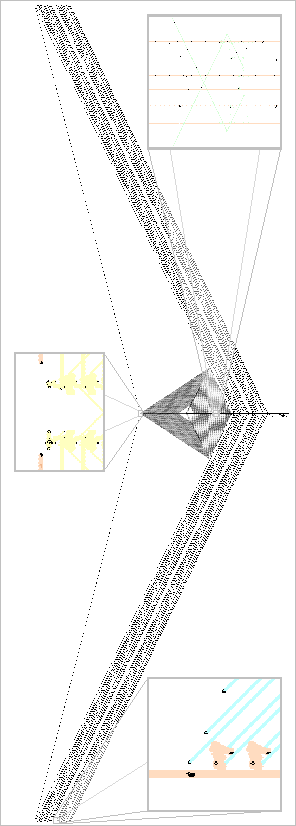
\includegraphics[width=\textwidth]{self_support_spaceships/shield_bug.pdf}}
			\caption{The \emph{shield bug}, travelling to the left.}\label{fig:shield_bug}
		\end{subfigure} &
		\begin{subfigure}{0.4267\textwidth}
			\centering
			\embedlink{centipede}{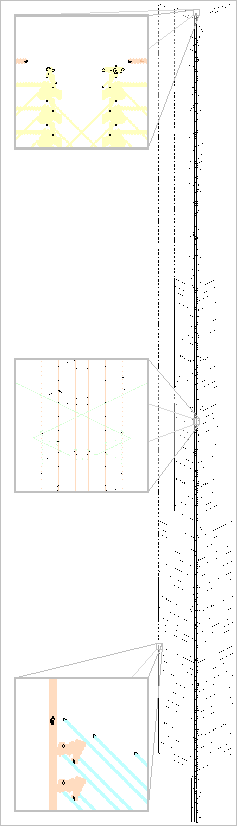
\includegraphics[width=\textwidth]{self_support_spaceships/centipede.pdf}}
			\caption{The \emph{centipede}, travelling up.}\label{fig:centipede}
		\end{subfigure}
	\end{tabular}
	\caption{A pair of (huge) $31c/240$ spaceships based on the same Herschel-crawling reaction as the silverfish. They each use six block tracks that carry Herschel-based rakes down their center, and the same double-HWSS slow salvo synthesis on their sides to stabilize the front end.}
	\label{fig:centipede_shield_bug}
\end{figure}

% 3c/10 reaction (ref figure in chapter 1), why it hasn't worked yet. See Dave's write-up at https://www.conwaylife.com/forums/viewtopic.php?f=15&t=3427

% 2014-present: self-supporting spaceships (half-baked knightship, waterbear, Centipede, Caterloopillar). The name "Caterloopillar" is something of a tribute to Douglas Hofstadter's "strange loop" concept. It's a deeply weird Life spaceship design where each half of the spaceship builds the other half as the whole thing is flying along, reminiscent of Escher's "Drawing Hands" lithograph.


%%%%%%%%%%%%%%%%%%%%%%%%%%%%%%%%%
\section*{Exercises \hfill \normalfont\textsf{\small solutions to starred exercises on \hyperlink{solutions_self_support_spaceships}{page \pageref{solutions_self_support_spaceships}}}}
\label{sec:solutions_self_support_spaceships}
\addcontentsline{toc}{section}{Exercises}
\vspace*{-0.4cm}\hrulefill\vspace*{-0.3cm}\footnotesize\begin{multicols}{2}\vspace*{-0.4cm}\raggedcolumns\interlinepenalty=10000
	\setlength{\parskip}{0pt}
	%%%%%%%%%%%%%%%%%%%%%%%%%%%%%%%%%
	
	
	\begin{problem}\label{exer:self_support_spaceships_track_layer_rephaser}
		There are some non-highlighted cells near the center of the block-laying pattern displayed in Figure~\ref{fig:31c_240_track_builder}. What is their purpose?
	\end{problem}
	% SOLUTION: They are a rephaser (really they are there since we will turn them into a forward rake in the completed silverfish, but for this exercise it's fine to just say that they adjust the lanes of the gliders so that the proper kickback/synthesis reactions happen).
	
	
	\mfilbreak
	
	
	\begin{problemstar}\label{exer:self_support_spaceships_r4l1}\index{double kickback}
		One way of creating rakes for Herschel crawlers (used by the silverfish) that output gliders on different lanes is to use a \emph{double kickback} reaction: the two-glider kickback reaction twice. For example, the\texttt{R6L17} rake from Figure~\ref{fig:R6L17} uses two double kickback reactions.
		
		\begin{enumerate}[label=\bf\color{ocre}(\alph*)]
			\item Modify the rake from Figure~\ref{fig:R6L17} so as to use just \emph{one} double kickback reaction.
			
			\item What is the name (in the \texttt{R\#L\#} format) of the rake that you created in part~(a)?
			
			\item Explain why the rake that you constructed in part~(a) is not useful when constructing the silverfish.
		\end{enumerate}
	\end{problemstar}
	
	
	\mfilbreak
	
	
	\begin{problem}\label{exer:self_support_spaceships_r6l21}
		Another forward rake that crawls along $6$~block tracks and could be used in the construction of the silverfish is displayed below.
		\begin{center}
			\gridbox{0.5pt}{\patternimglink{0.063}{R6L21}}
		\end{center}
		
		\begin{enumerate}[label=\bf\color{ocre}(\alph*)]
			\item What is the name (in the \texttt{R\#L\#} format) of this rake?
			% R6L21
			
			\item Explain why this rake is not useful when constructing the silverfish.
			% L21 is more efficiently reached by R2L25 + 3.
		\end{enumerate}
	\end{problem}
	
	
	\mfilbreak
	
	
	\begin{problemstar}\label{exer:self_support_spaceships_r2l16}
		In this exercise, we create another rake that crawls along $6$~block tracks and could be used in the construction of the silverfish.
		
		\begin{enumerate}[label=\bf\color{ocre}(\alph*)]
			\item Adjust the positions of the two outermost Herschels in the rephaser from Figure~\ref{fig:31c_240_rephaser} so that the gliders on the outside of the tracks do not annihilate each other. Doing so should create a forward-and-backward rake.
			
			\item Place the forward rake \texttt{R1L0} behind the double rake that you created in part~(a) so as to eliminate its backward gliders.
			
			\item What is the name (in the \texttt{R\#L\#} format) of the rake that you created in part~(b)?
			%R2L16
			
			\item Explain why the rake that you constructed in part~(b) is not useful when constructing the silverfish.
			
			[Hint: Be careful. The answer is slightly different than it was in Exercises~\ref{exer:self_support_spaceships_r4l1} and~\ref{exer:self_support_spaceships_r6l21}.]
		\end{enumerate}
	\end{problemstar}
	
	
	
	\mfilbreak
	
	
	\begin{problem}\label{exer:self_support_spaceships_r3l28}
		Another forward rake that crawls along $6$~block tracks and could be used in the construction of the silverfish is displayed below.
		\begin{center}
			\gridbox{0.5pt}{\patternimglink{0.11}{R3L28}}
		\end{center}
		
		\begin{enumerate}[label=\bf\color{ocre}(\alph*)]
			\item What is the name (in the \texttt{R\#L\#} format) of this rake?
			% R3L28
			
			\item Create an updated version of Table~\ref{tab:silverfish_forward_rakes} that takes this rake into account. Which rake from Figure~\ref{fig:31c_240_forerakes} is no longer useful in the construction of the silverfish?
			% Table: https://www.conwaylife.com/forums/viewtopic.php?f=2&t=1274&start=375#p98852
			% R6L6
			
			\item On page~\pageref{page:silverfish_rake_seq}, we gave a sequence of rakes that would fire 13 gliders as efficiently as possible using the rakes we had at that time. Update this sequence now that we have this new rake.
			% Also https://www.conwaylife.com/forums/viewtopic.php?f=2&t=1274&start=375#p98852
			
			\item Reconstruct the silverfish according to the sequence of rakes that you compiled in part~(c).
			
			[Hint: Most of the silverfish from Figure~\ref{fig:silverfish} can be left as-is. All that needs to be changed is which rakes crawl along its central block tracks.]
		\end{enumerate}
	\end{problem}
	
	
	\mfilbreak
	
	
	\begin{problem}\label{exer:silverfish_list_of_lanes}
		On page~\pageref{page:silverfish_lanes} we listed a sequence of mod~$31$ lane numbers for implementing the slow salvo synthesis from Figure~\ref{fig:hwss_from_toad_beehive}. The list of lanes that can be used is actually much more flexible than indicated there. For example, we can fire the first two gliders on lanes $0$ and $11$ in either order, since the first two gliders in that slow salvo do not interact with each other.
		
		Provide a complete description of all possible sequences of mod~$31$ lane numbers that implement the synthesis from Figure~\ref{fig:hwss_from_toad_beehive}.
	\end{problem}
	% Solution: (0 and 11 in either order), 8, 7, (29 and 13 in either order), 1, (15 or 16 or 19 or 26), 8, 0, 14, 22, (1 or 2 or 3 or 4 or 5 or 6)
	
	
	\mfilbreak
	
	
	\begin{problem}\label{exer:silverfish_backward_glider_destroy}
		Two of the gliders from the slow salvo synthesis of Figure~\ref{fig:hwss_from_toad_beehive} are just used to destroy a beehive and a block.
		
		\begin{enumerate}[label=\bf\color{ocre}(\alph*)]
			\item Adjust the synthesis so that those two gliders come from the northwest instead of the northeast.
			
			\item Construct a silverfish that is at least 100 rows shorter than the one from Figure~\ref{fig:silverfish} by using a backrake to produce one or both of the gliders that were repositioned in part~(a).
			
			[Hint: A rephaser from near the front of the silverfish can be turned into a backrake whose stream crosses that of the forward rakes.]
		\end{enumerate}
	\end{problem}
	% SOLUTION: https://www.conwaylife.com/forums/viewtopic.php?f=2&t=1274&start=375#p98847
	
	
	\mfilbreak
	
	
	\begin{problem}\label{exer:pi_forward_rake_break_apart}
		Break down the forward rake from Figure~\ref{fig:pi_forward_rake}, which is made up of six pi crawlers, into separate non-interacting pieces that each consist of fewer pi crawlers.
	\end{problem}
	
	%% EXERCISE END COMMANDS
\end{multicols}
\normalsize\vspace*{0.01cm}
%% DONE EXERCISE END COMMANDS